\documentclass[border=2mm,12pt,tikz]{standalone}
\usepackage{tikz-3dplot} 
\usepackage{bm}
\usepackage{pgfplots}
\usepackage{graphicx}

\usetikzlibrary{intersections,patterns.meta}
\begin{document}
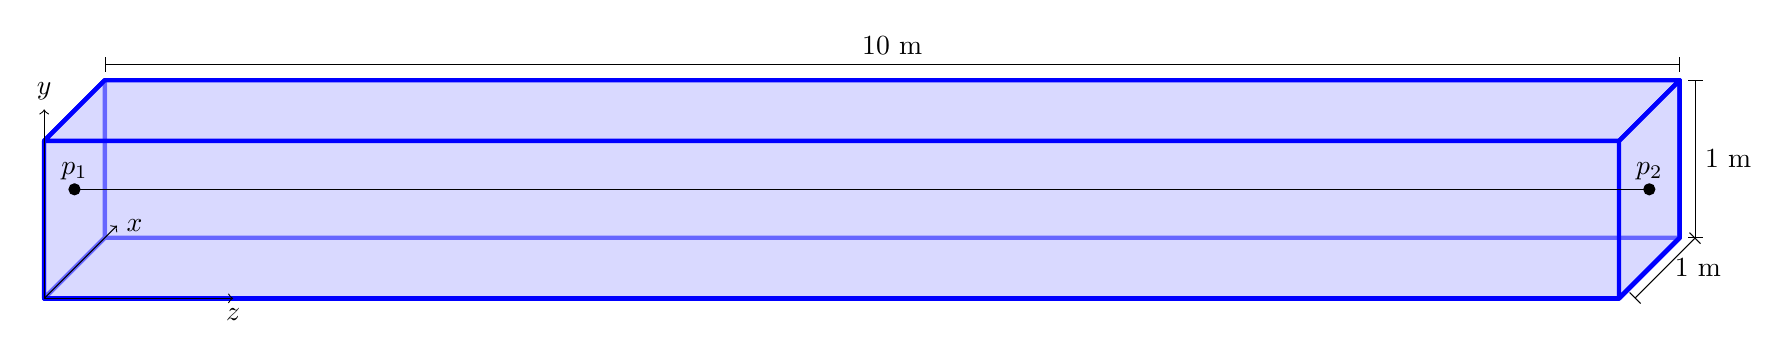
\begin{tikzpicture}[
        scale = 2, 
        line join=round,
        mystyle/.style = {ultra thick, blue, fill=blue!20, fill opacity=0.5},
        rotate around y=90
    ]

    \coordinate (1) at (0,0,0);
    \coordinate (2) at (0,1,0);
    \coordinate (3) at (1,1,0);
    \coordinate (4) at (1,0,0);

    \coordinate (5) at (0,0,10);
    \coordinate (6) at (0,1,10);
    \coordinate (7) at (1,1,10);
    \coordinate (8) at (1,0,10);


    % desenhando todas as faces um paralelepípedo com os vértices dados

    \draw[mystyle] (1) -- (2) -- (3) -- (4) -- cycle;
    \draw[mystyle] (3) -- (4) -- (8) -- (7) -- cycle;
    \draw[mystyle] (4) -- (1) -- (5) -- (8) -- cycle;
    \draw[mystyle] (1) -- (2) -- (6) -- (5) -- cycle;
    \draw[mystyle] (2) -- (3) -- (7) -- (6) -- cycle;
    \draw[mystyle] (5) -- (6) -- (7) -- (8) -- cycle;

    \draw[->] (0, 0, 0) -- (1.2, 0, 0) node[right] {$x$};
    \draw[->] (0, 0, 0) -- (0, 1.2, 0) node[above] {$y$};
    \draw[->] (0, 0, 0) -- (0, 0, 1.2) node[below] {$z$};

    \draw[|-|] (3) ++ (0, 0.1, 0) --++ (0,0,10) node[midway, above] {$10$ m};
    \draw[|-|] (8) ++ (0, 0, 0.1) --++ (0,1,0) node[midway, right] {$1$ m};
    \draw[|-|] (5) ++ (0, 0, 0.1) --++ (1,0,0) node[midway, right] {$1$ m};
    
    \coordinate (p2) at (0.5,0.5,10);
    \coordinate (p1) at (0.5,0.5,0);
    \filldraw[black] (p2) circle (1pt) node[above] {$p_2$};
    \filldraw[black] (p1) circle (1pt) node[above] {$p_1$};
    \draw (p1) -- (p2);

\end{tikzpicture}
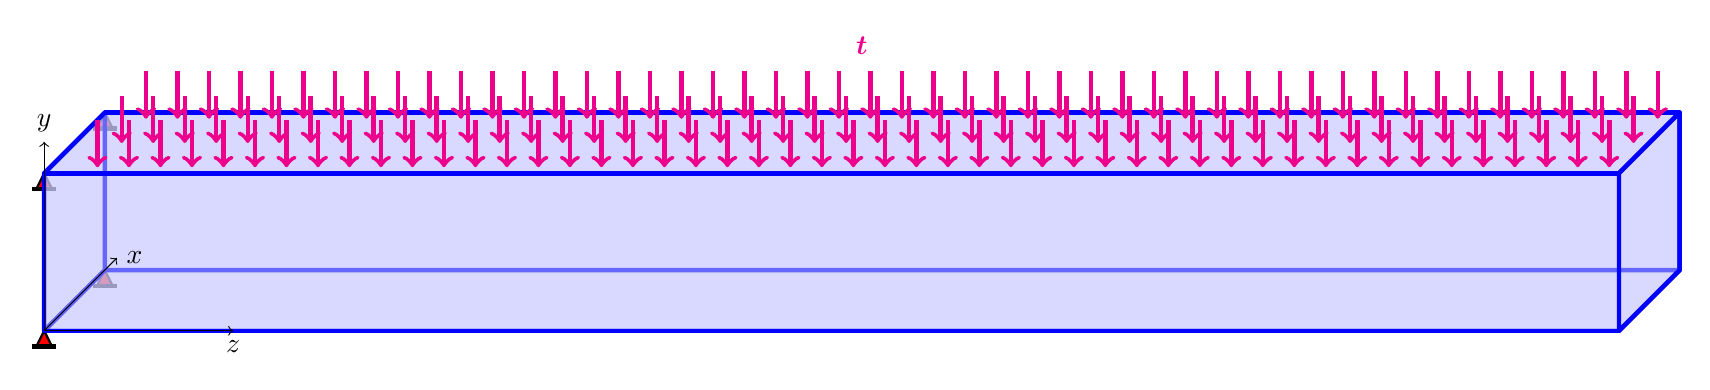
\begin{tikzpicture}[
    scale = 2, 
    line join=round,
    mystyle/.style = {ultra thick, blue, fill=blue!20, fill opacity=0.5},
    rotate around y=90
]

    \coordinate (1) at (0,0,0);
    \coordinate (2) at (0,1,0);
    \coordinate (3) at (1,1,0);
    \coordinate (4) at (1,0,0);

    \coordinate (5) at (0,0,10);
    \coordinate (6) at (0,1,10);
    \coordinate (7) at (1,1,10);
    \coordinate (8) at (1,0,10);

    \draw[thick, fill = red] (2) --++ (0, -0.1, 0.05) --++ (0, 0, -0.1) -- cycle;
    \draw[ultra thick] (2) ++ (0, -0.1, 0.075) --++ (0, 0, -0.15);
    \draw[thick, fill = red] (3) --++ (0, -0.1, 0.05) --++ (0, 0, -0.1) -- cycle;
    \draw[ultra thick] (3) ++ (0, -0.1, 0.075) --++ (0, 0, -0.15);
    \draw[thick, fill = red] (4) --++ (0, -0.1, 0.05) --++ (0, 0, -0.1) -- cycle;
    \draw[ultra thick] (4) ++ (0, -0.1, 0.075) --++ (0, 0, -0.15);
    \draw[thick, fill = red] (1) --++ (0, -0.1, 0.05) --++ (0, 0, -0.1) -- cycle;
    \draw[ultra thick] (1) ++ (0, -0.1, 0.075) --++ (0, 0, -0.15);

    % desenhando todas as faces um paralelepípedo com os vértices dados

    \draw[mystyle] (1) -- (2) -- (3) -- (4) -- cycle;
    \draw[mystyle] (3) -- (4) -- (8) -- (7) -- cycle;
    \draw[mystyle] (4) -- (1) -- (5) -- (8) -- cycle;
    \draw[mystyle] (1) -- (2) -- (6) -- (5) -- cycle;
    \draw[mystyle] (2) -- (3) -- (7) -- (6) -- cycle;
    \draw[mystyle] (5) -- (6) -- (7) -- (8) -- cycle;

    \draw[->] (0, 0, 0) -- (1.2, 0, 0) node[right] {$x$};
    \draw[->] (0, 0, 0) -- (0, 1.2, 0) node[above] {$y$};
    \draw[->] (0, 0, 0) -- (0, 0, 1.2) node[below] {$z$};


    \foreach \z in {0.3, 0.5, ..., 9.9} {
        \foreach \x in {0.1, 0.5, ..., 0.9} {
            \draw[<-, magenta, ultra thick] (\x, 1, \z) --++ (0, 0.3, 0);
        }
    }
    \draw (0.5, 1.5, 5) node[above, magenta] {$\bm{t}$};

\end{tikzpicture}

\begin{tikzpicture}
   \begin{axis}[
        xlabel={$x$ ao longo de $\overline{p_1 p_2}$ [m]},
        ylabel = {Deslocamento em $y$},
        grid,
        xmin=0,xmax=10,
        grid style={dotted},
        width= 20cm,
        height= 10cm,
        title={Deslocamento vertical ao longo do centro da viga}
        ]
      
        \addplot [blue, sharp plot, thick] table {../../validation/1 verification case.dat};
        \addlegendentry{PHILLIPO.jl};
        \addplot[domain = 0:10]{-1e6 * 12 / 210e9 / 24 * \x^2 * (6 * 10^2 - 4 * 10 * \x + \x^2) };
        \addlegendentry{Solução analítica $y(x) = \frac{t_0}{EI} \frac{Lx^2}{24} \left(6L^2 - 4Lx+x^2\right)$};
    \end{axis}
\end{tikzpicture}

\end{document} 